\section{Experiments}\label{sec:experiments}

We evaluate temporal probes across four reasoning models (\cref{tab:models}), comparing hidden-state (HS) and text modalities under different layer selection criteria.

\subsection{Setup}\label{sec:setup}

We study R1-8B (Llama-8B, R1-distilled, $n{=}43$ test traces), OT-7B (OpenThinker-7B, trained on the OpenThoughts dataset~\citep{openthinker}; Qwen-7B backbone, STILL-trained~\cref{app:ot7b_details}, $n{=}47$), QwQ-32B (Qwen-32B, native reasoning, $n{=}19$--$20$), and R1-32B (Qwen-32B, R1-distilled, $n{=}20$). All traces come from HarmThoughts with step-level CP annotations (60/20/20 split). HS probes extract last-token hidden states from a selected layer; text probes encode each step with all-MiniLM-L6-v2 (384d). Both use L2-regularized logistic regression with temporal windowing $W \in \{1, 3, 5, 10, 15, 20, 25\}$ selected on validation. Classification requires $K{=}5$ consecutive threshold crossings (\cref{tab:k_ablation}). Statistical testing follows \cref{sec:evaluation}.\looseness=-1

\subsection{Layer Selection Results}\label{sec:layer-results}

\cref{tab:layer_selection} shows that the CR-composite systematically selects shallow layers: L0 for R1-8B (full L0--L24 sweep; \cref{tab:r18b_full_layer}) and OT-7B, L2 (3\%) for QwQ-32B, L10 (16\%) for R1-32B (\cref{fig:layer_heatmap}). Threshold-based metrics converge to deep layers, notably L63 (98\%) for both 32B models. Balanced accuracy varies across splits (7--98\% depth; \cref{app:ba_layer_comparison}). The mechanism is cosine compression: step-to-step distances are 1.4--2.7$\times$ smaller at shallow layers (\cref{app:cosine_volatility}), so a linear probe operates near the noise floor, inflating crossing rate independently of discriminative power (\cref{sec:layer-sensitivity}).\looseness=-1

\begin{table}[t]
\centering
\small
\resizebox{\columnwidth}{!}{%
\begin{tabular}{lcccc}
\toprule
\textbf{Model} & \textbf{CR-comp.}$^a$ & \textbf{Thresh.}$^b$ & $p$ \textbf{(thresh.)} & $\Delta$\textbf{Prec}$^c$ \\
\midrule
R1-8B & L0 (0\%) & L14 (44\%) & ${<}0.001$ & +20.1 \\
OT-7B & L0 (0\%) & L16 (57\%) & ${<}0.001$ & +21.9 \\
QwQ-32B$^\dagger$ & L2 (3\%) & L63 (98\%) & ${<}0.005$ & +19.2 \\
R1-32B$^\dagger$ & L10 (16\%) & L63 (98\%) & ${<}0.001$ & +15.4 \\
\bottomrule
\end{tabular}}
\caption{Layer selection sensitivity. $^a$\,Crossing-rate composite (bal\_acc $\times$ crossing\_rate). $^b$\,Consensus of threshold-based metrics (precision, inverse FPR, additive composite). $^c$\,HS$-$text precision difference (pp) at threshold-based layer (\cref{tab:hs_vs_text}). Rightmost $p$: HS vs.\ text precision $p$-value at threshold-based layer (e.g., QwQ-32B CR-composite layer: $p{=}0.83$, non-significant). $\dagger$\,Sample-limited ($n \leq 20$).}
\label{tab:layer_selection}
\end{table}

\begin{figure}[t]
\centering
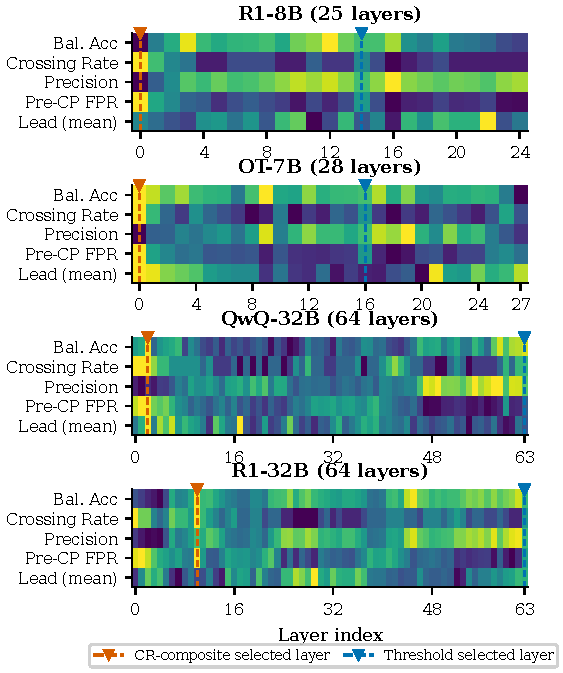
\includegraphics[width=\columnwidth]{figures/fig_layer_heatmap.pdf}
\caption{Per-layer metric heatmap (2$\times$2). Each column: one of five metrics (balanced accuracy, precision, inverse FPR, crossing rate, additive composite; min-max normalized). Red dashed: CR-composite layer (bal\_acc $\times$ crossing\_rate); green dashed: threshold-based layer (consensus of threshold-based metrics). For R1-8B (full L0--L24 sweep), crossing rate drives CR-composite selection to L0 while threshold-based metrics retain L14. At 32B, CR-composite selections cluster near input layers while threshold-based metrics peak at deep layers.}
\label{fig:layer_heatmap}
\end{figure}

The downstream impact is severe: at CR-composite layers, only 7--8B models show significant HS advantage; both 32B models fail. CR-composite shallow-layer selection is an artifact of cosine compression, not a genuine safety signal. At threshold-based layers, the HS advantage is graded: cross-validated at 7--8B, significant at QwQ-32B, and exploratory at R1-32B (small sample). Random-label controls confirm threshold-based selection requires genuine safety labels and that the geometric bias is Qwen-specific (\cref{app:random_cp}). AUROC confirms HS discriminability at balanced-accuracy-selected layers ($\Delta$AUROC +12--15pp; \cref{tab:ba_layer_results}) but cannot diagnose threshold-dependent bias.\looseness=-1

\paragraph{Ensemble layer selection.} A three-layer ensemble averaging predictions from the precision-best, balanced-accuracy-best, and inverse-FPR-best layers bypasses single-metric selection. All four models show significant HS advantage ($p \leq 0.002$; \cref{tab:ensemble}), including both 32B models that fail under CR-composite. The ensemble smooths metric-specific variation by averaging across depths within the deep region. This holdout result requires cross-validated confirmation (\cref{sec:discussion}).\looseness=-1

\begin{figure}[t]
\centering
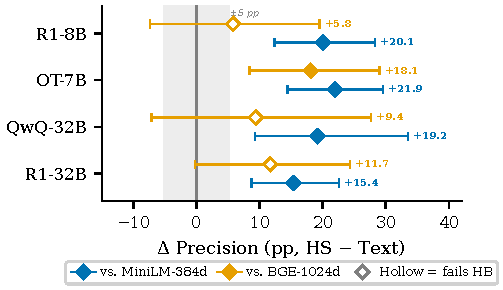
\includegraphics[width=\columnwidth]{figures/fig_forest_precision.pdf}
\caption{HS precision advantage (pp) over text probes with 95\% bootstrap CI. Blue: vs.\ MiniLM-384d; orange: vs.\ BGE-1024d. Solid: survives Holm--Bonferroni correction; hollow: does not. The encoder-quality gradient is monotonic: all 384d comparisons significant; at 1024d only OT-7B survives.}
\label{fig:forest_precision}
\end{figure}

\begin{table}[t]
\centering
\small
\caption{Multi-metric layer ensemble vs.\ best single metric and text baseline. Ensemble trains probes at 3 threshold-based metric-selected layers and averages probabilities. $\Delta$Ens--Best: ensemble minus best single metric (negative = ensemble slightly lower). All Ens--Text differences are significant ($p \leq 0.002$, permutation test). No Ens--Best difference is significant ($p > 0.27$).}
\label{tab:ensemble}
\resizebox{\columnwidth}{!}{%
\begin{tabular}{lcccc}
\toprule
\textbf{Model} & \textbf{Ens Prec} & \textbf{Best Single} & $\Delta$ & \textbf{Ens$-$Text} \\
\midrule
R1-8B & 0.565 & 0.604 (BA@L12) & $-$3.9pp & +19.3pp \\
OT-7B & 0.506 & 0.473 (FPR@L18) & +3.3pp & +27.0pp \\
QwQ-32B & 0.578 & 0.578 (Prec@L60) & $-$0.0pp & +20.3pp \\
R1-32B & 0.581 & 0.583 (Prec@L63) & $-$0.2pp & +10.5pp \\
\bottomrule
\end{tabular}}
\end{table}

\paragraph{Cross-dataset replication (AdvBench).} We replicate the five-metric layer sweep on AdvBench~\citep{advbench} (520 traces, 159 jailbreaks, R1-8B, binary labels). The CR-composite selects shallow layers (median L2) while precision selects deep (median L14), a 31.7pp divergence (95\% CI [3.2, 48.4]pp, $p{=}0.015$; 1{,}000 bootstrap iterations) consistent with HarmThoughts. This confirms layer selection bias (C1) is geometric, not label-dependent; AdvBench does not validate C2 (\cref{app:advbench_layer_bias,app:advbench_cp}).\looseness=-1

\subsection{HS vs.\ Text Comparison}\label{sec:hs-text}

Against the 384d text baseline, HS probes outperform text in all four models (\cref{tab:hs_vs_text}). The advantage is cross-validated at 7--8B (R1-8B: +20.1pp, OT-7B: +21.9pp precision) and consistent across random seeds (\cref{app:multi_seed}). At 32B, results are suggestive: QwQ-32B shows +19.2pp but the position baseline is competitive (\cref{sec:32b-analysis}); R1-32B shows +15.4pp but with limited coverage. Control tasks confirm the signal reflects genuine safety structure (\cref{app:control}); a split-half analysis on OT-7B confirms internal validity (\cref{app:split_half}).\looseness=-1

\paragraph{Capacity control.} PCA reduction of HS features to 384d (79--92\% variance retained) preserves the precision advantage across all four models (+16.8 to +23.1pp, all $p{<}0.012$, all survive correction). The control provides partial evidence against a pure capacity explanation. Random projection to 384d yields similar results ($\Delta$Prec +8.3 to +20.5pp; \cref{app:random_projection}), further weakening the capacity explanation. E5-Mistral-7B (4096d, PCA-reduced to 384d; \cref{app:e5_mistral}) yields intermediate results (2/4 significant), forming a monotonic encoder-quality gradient with MiniLM (4/4) and BGE-large (1/4).\looseness=-1

\paragraph{Encoder robustness.} The HS advantage is encoder-conditional. Against BGE-large~\citep{xiao2023cpack} (1024d), only OT-7B survives correction (1/4 precision; \cref{app:encoder_robustness}). \cref{fig:forest_precision} visualizes the encoder-quality gradient: MiniLM-384d (4/4 significant) $\to$ E5-Mistral (2/4) $\to$ BGE-1024d (1/4), with precision narrowing from +15--22pp to +6--18pp. Layer selection bias (C1) is encoder-independent.\looseness=-1

\paragraph{Position mediation.} Position ($t/T$) accounts for 12--20pp of balanced accuracy, but all models retain non-positional signal above chance (\cref{app:position_residual}). Under linear residualization, 3/4 models retain significant non-positional HS advantage; quadratic residualization absorbs the advantage in 2/4 models (\cref{tab:position_quadratic}). Per-model residualization details appear in \cref{sec:discussion}. Temporal windowing reduces position dependence (\cref{sec:temporal}).\looseness=-1

\begin{table*}[t]
\centering
\small
\begin{tabular}{llclrrlrc}
\toprule
\textbf{Model} & \textbf{Layer} & \textbf{Enc.} & $W$ & $\Delta$\textbf{BA} & $\Delta$\textbf{Prec} & \textbf{95\% CI} & $\Delta$\textbf{FPR} & \textbf{HB} \\
\midrule
R1-8B & L14 & 384d & 3 & +17.5 & +20.1 & [+12.4, +28.3] & $-$7.9 & \checkmark \\
 & & 1024d & & \multicolumn{1}{c}{--} & +5.8 & [$-$7.4, +19.5] & \multicolumn{1}{c}{--} & \\[2pt]
OT-7B & L16 & 384d & 3 & +10.7 & +21.9 & [+14.0, +29.6] & $-$17.1 & \checkmark \\
 & & 1024d & & \multicolumn{1}{c}{--} & +18.1 & [+8.4, +29.0] & \multicolumn{1}{c}{--} & \checkmark \\[2pt]
QwQ-32B$^\dagger$ & L63 & 384d & 5 & +13.0 & +19.2 & [+9.3, +33.5] & $-$15.0 & \checkmark \\
 & & 1024d & & \multicolumn{1}{c}{--} & +9.4 & [$-$7.1, +27.7] & \multicolumn{1}{c}{--} & \\[2pt]
R1-32B$^\dagger$ & L63 & 384d & 1 & +18.7 & +15.4 & [+8.7, +22.6] & $-$14.6 & \checkmark \\
 & & 1024d & & \multicolumn{1}{c}{--} & +11.7 & [$-$0.2, +24.3] & \multicolumn{1}{c}{--} & \\
\bottomrule
\end{tabular}
\caption{HS vs.\ text at threshold-based layers (logistic regression probes, 60/20/20 split, 10{,}000 bootstrap resamples). Enc.: text encoder (384d = MiniLM-L6-v2, 1024d = BGE-large). $\Delta$: HS$-$text difference (pp); ``--'' = BA and FPR are not computed for the 1024d comparison because the 384d and 1024d encoders operate at different probe calibration points and do not share a decision threshold. HB: \checkmark{} = model-level test passes Holm-Bonferroni ($\alpha{=}0.05$); all 384d model-level tests pass. $^\dagger$\,Sample-limited ($n \leq 20$); 32B results are suggestive. 1024d: Holm--Bonferroni over 4 model-level precision tests.}
\label{tab:hs_vs_text}
\end{table*}

\subsection{32B Scale}\label{sec:32b-analysis}

Results at 32B are suggestive due to small test sets ($n{=}19$--$20$; \cref{app:power_analysis}). The two models present divergent profiles despite sharing the Qwen-32B architecture. R1-32B suggests early commitment detection ($W{=}1$ only, 25\% coverage, +14.2pp over position baseline), but the residualized hidden-state--text gap (+1.9pp) is not significant, consistent with position mediation. QwQ-32B achieves significance at all window sizes (74\% coverage) but with negative lead time ($-$1.2 to +1.9 steps); the position baseline is competitive (balanced accuracy 0.832 vs.\ 0.796, not significant). Neither model provides confirmatory evidence; replication with $n \geq 50$ traces is needed. Full analysis in \cref{app:32b_full}.\looseness=-1

\subsection{Temporal Context}\label{sec:temporal}

Temporal windowing ($W{>}1$) improves both modalities (\cref{fig:window_ablation}): at 7--8B, the modality advantage (+20.1 to +21.9pp) exceeds temporal improvement (+13pp). GRU models achieve comparable accuracy but higher FPR (\cref{tab:gru_multi_seeds,app:temporal_details}); an adaptive two-stage strategy offers marginal gains (\cref{app:two_stage}). CP-aligned probe trajectories confirm sharper HS transitions at the commitment point (\cref{fig:trajectory}).\looseness=-1

\begin{figure}[t]
\centering
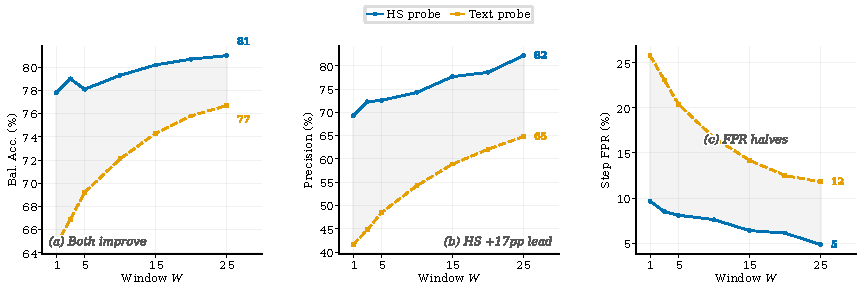
\includegraphics[width=\columnwidth]{figures/fig2_temporal_improvement.pdf}
\caption{Temporal window effect on R1-8B HS probe (L14). Precision: 69.3\% ($W{=}1$) to 82.2\% ($W{=}25$); FPR: 9.65\% to 4.83\%.}
\label{fig:window_ablation}
\end{figure}

\subsection{Negative Results}\label{sec:negative}

No alternative method consistently matches supervised probing (\cref{tab:negative}). BOCPD~\citep{adams2007bayesian}/CUSUM fail (0\% detection on 3/4 models); Mahalanobis yields near-zero separation; RepE~\citep{zou2023representation} is model-dependent (BA 0.756 vs.\ 0.559); MLP probes overfit; CCS misaligns temporally; cross-model transfer fails (\cref{app:negative_details}). Per-model failure analysis (\cref{app:negative_details}) identifies mechanism-specific causes: BOCPD sensitivity to $\lambda$ prior, Mahalanobis collapse under high-dimensional HS, and CCS temporal misalignment. The signal is directional, gradual, model-specific, and linearly separable, excluding change-point, distance, transfer, and objective-alignment methods.\looseness=-1

\begin{table}[t]
\centering
\small
\resizebox{\columnwidth}{!}{%
\begin{tabular}{p{1.4cm}p{2.5cm}p{2.0cm}p{1.6cm}}
\toprule
\textbf{Method} & \textbf{Result} & \textbf{Limitation} & \textbf{Failure Cat.} \\
\midrule
BOCPD & 0\% det.\ on 3/4 models & Commitment gradual & Graduality \\
CUSUM & $<$ threshold, all models & Same as BOCPD & Graduality \\
Mahalanobis & $\Delta d \approx 0$ & Signal in minor PCs & Var.\ subspace \\
RepE & QwQ 0.756; R1-32B 0.559$^a$ & Model-dependent & Model-spec. \\
MLP & 3/4 worse than LR & Overfitting & Capacity \\
CCS & No gain over supervised$^b$ & Alignment mismatch & Obj.\ mismatch \\
Transfer & Best 59.5\% (PCA)$^c$ & Model-specific repr. & Model-spec. \\
\bottomrule
\end{tabular}}
\caption{Seven alternative approaches. $^a$\,RepE QwQ approaches supervised bal\_acc but precision is 0.512 vs.\ LR 0.700. $^b$\,Semi-supervised (requires CP labels). $^c$\,Best direct transfer 67.3\% but 1\% crossing rate.}
\label{tab:negative}
\end{table}

\begin{figure}[t]
\centering
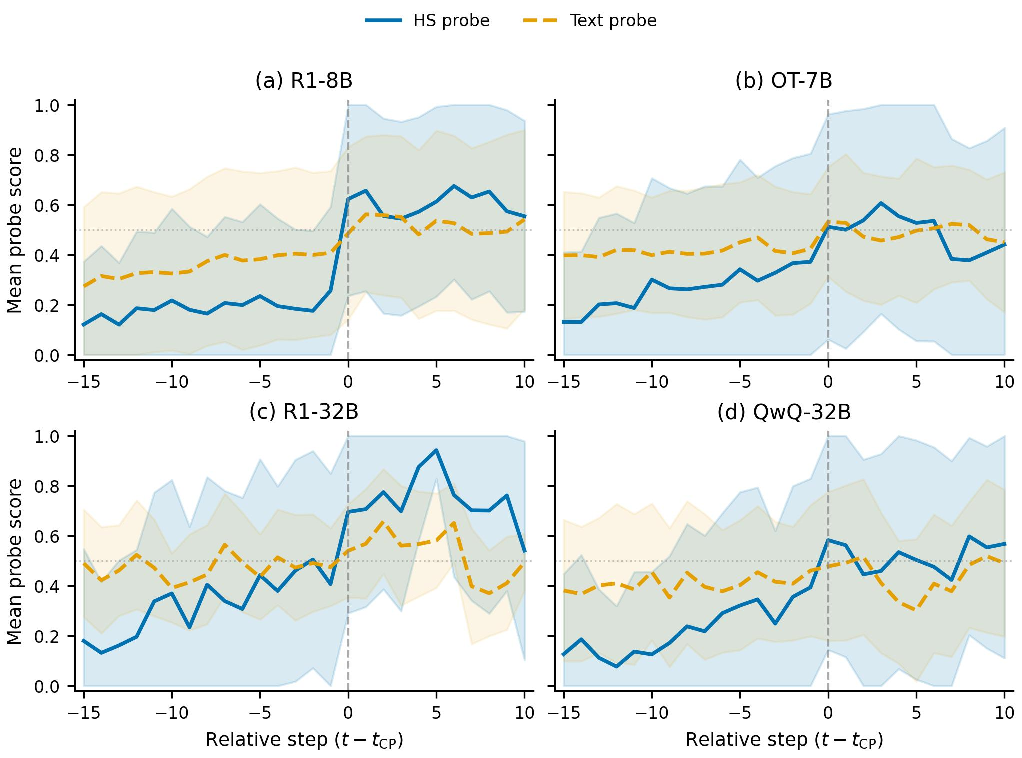
\includegraphics[width=\columnwidth]{figures/fig_trajectory.pdf}
\caption{CP-aligned probe score trajectories. Each panel averages all test traces for one model, with step 0 at the true commitment point. HS probes (blue, solid) show a sharper score increase at CP than text probes (orange, dashed), with OT-7B showing the strongest separation and R1-32B the weakest, consistent with the evidence gradient. Shaded bands: $\pm$1 std. Points with $<$5 traces are omitted.}
\label{fig:trajectory}
\end{figure}
